\chapter{Friedmann-Dynamik: Materie, Strahlung und Vakuumenergie}

\lectureoverview{Die Kinematik eines expandierenden Universums lässt sich in einer Zeile ausdrücken: Physikalische Abstände wachsen mit einem Skalenfaktor \(a(t)\). Nun müssen wir diese Funktion bestimmen. Wir leiten die Friedmann-Gleichung für den flachen Raum aus der Newtonschen Energieerhaltung her, lösen sie zunächst für gewöhnliche Materie und sehen dann, warum Strahlung und Vakuumenergie zu völlig anderen kosmischen Entwicklungsgeschichten führen.}

\section{Die zu erklärende Geometrie}

Zu einem festen kosmischen Zeitpunkt erscheint das Universum auf großen Skalen homogen und isotrop. Galaxien, Galaxienhaufen und Superhaufen sind durchaus reale Strukturen, doch auf Skalen von Hunderten Millionen oder Milliarden Lichtjahren wird ihre Verteilung bemerkenswert gleichförmig. Diese empirische Regelmäßigkeit heißt kosmologisches Prinzip. Der Name macht sie nicht zu einem Satz; ihre Aussagekraft beruht auf Beobachtungen.

Es gibt eine zweite empirische Tatsache. Innerhalb der heutigen Messgenauigkeit verhalten sich große räumliche Dreiecke wie euklidische Dreiecke. Der Vergleich mit einer Vermessung eines Fußballfelds ist hilfreich. Wenn straff gespannte Linien Dreiecke bilden, deren Winkel sich zu \(180^\circ\) summieren, hat man damit nicht bewiesen, dass die Erde global flach ist. Man hat gezeigt, dass ihr Krümmungsradius groß gegenüber dem Spielfeld ist. Die kosmische Vermessung folgt derselben Logik: Der Raum kann einen sehr großen Krümmungsradius haben, lässt sich im beobachtbaren Bereich aber gut als flach annähern.

Die Referenzgeometrie ist die Minkowski-Raumzeit,
\begin{equation}
  d\tau^2=dt^2-\left(dx^2+dy^2+dz^2\right).
  \label{eq:l09-minkowski}
\end{equation}
Die Klammer bezeichnet schlicht das euklidische Linienelement im dreidimensionalen Raum. In der Allgemeinen Relativitätstheorie sind die Koeffizienten der Koordinatendifferentiale dagegen Felder. Sie können sich mit Ort und Zeit ändern; auch gemischte Terme können auftreten. Diese Metrikkoeffizienten sind die relativistischen Nachfolger des Newtonschen Gravitationsfelds.

\begin{figure}[H]
  \centering
  \includegraphics[width=0.72\textwidth]{lecture_09_figure_01.png}
  \caption{Das zu Beginn der Vorlesung angegebene Minkowski-Eigenzeitelement. Quellbild bei 00:01:50.}
  \label{fig:l09-minkowski-board}
\end{figure}

Für ein räumlich flaches, expandierendes Universum lassen Homogenität und Isotropie nur einen zeitabhängigen Skalenfaktor zu:
\begin{equation}
  d\tau^2=dt^2-a^2(t)\left(dx^2+dy^2+dz^2\right).
  \label{eq:l09-flat-frw}
\end{equation}
Wir verwenden Einheiten, in denen \(c=1\) gilt, sodass Zeit und Länge dieselbe Dimension haben. Es gibt zwei konsistente Konventionen. Man kann \(x,y,z\) die Dimension einer Länge geben und \(a\) dimensionslos wählen, oder \(x,y,z\) als dimensionslose Bezeichnungen behandeln und \(a\) die Dimension einer Länge zuweisen. Die Vorlesung verwendet die zweite Konvention, weil sie die physikalische Bedeutung von \(a(t)\) sichtbar macht.

\begin{figure}[H]
  \centering
  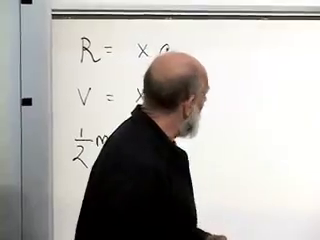
\includegraphics[width=0.72\textwidth]{lecture_09_figure_02.png}
  \caption{Die Metrik des flachen, expandierenden Universums, in der der Skalenfaktor das euklidische räumliche Linienelement multipliziert. Quellbild bei 00:09:12.}
  \label{fig:l09-expanding-metric-board}
\end{figure}

Stellen wir uns Koordinaten vor, die auf ein Gummituch gemalt sind. Die Koordinatenmarkierungen bleiben am Tuch haften, während der physikalische Abstand zwischen ihnen wächst. Eine Koordinatendifferenz wie „von \(x=0\) bis \(x=1\)“ ist also lediglich ein Paar von Bezeichnungen. Der durch dieses Intervall dargestellte Abstand beträgt \(a(t)\). Die Gleichung zu finden, die diesen Skalenfaktor bestimmt, ist das dynamische Problem dieser Vorlesung.

\section{Geschlossene, flache und offene räumliche Geometrien}

Flachheit ist eine beobachtungsbasierte Vereinfachung und folgt nicht aus der Homogenität. Es gibt drei homogene und isotrope räumliche Geometrien: mit positiver, verschwindender und negativer Krümmung. Um den Fall positiver Krümmung zu verstehen, muss man die Dimension genau beachten.

Der geometrische Ort
\begin{equation}
  X_1^2+X_2^2=R^2
\end{equation}
ist ein Kreis oder eine Einsphäre \(S^1\). Sein ausgefülltes Inneres ist eine Kreisscheibe, auch Zweikugel genannt. Fügt man eine Einbettungskoordinate hinzu, erhält man
\begin{equation}
  X_1^2+X_2^2+X_3^2=R^2,
\end{equation}
die gewöhnliche Zweisphäre \(S^2\). Mit einer vierten Einbettungskoordinate erhält man
\begin{equation}
  X_1^2+X_2^2+X_3^2+X_4^2=R^2,
  \label{eq:l09-three-sphere}
\end{equation}
eine Dreisphäre \(S^3\), die selbst ein dreidimensionaler Raum ist. Wir können ihre Einbettung in vier Dimensionen nicht veranschaulichen, doch ihre intrinsische Geometrie benötigt diese Einbettung nicht, um zu existieren.

\begin{figure}[H]
  \centering
  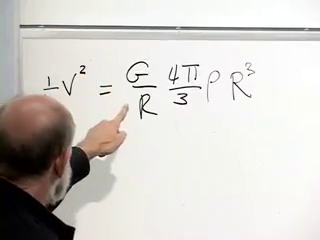
\includegraphics[width=0.72\textwidth]{lecture_09_figure_03.png}
  \caption{Die Einbettungsgleichung, mit der die Dreisphäre eingeführt wird. Quellbild bei
  00:16:40.}
  \label{fig:l09-three-sphere-board}
\end{figure}

Jeder Punkt einer idealen Sphäre ist geometrisch jedem anderen gleichwertig, und an jedem Punkt sind alle Richtungen gleichwertig. Eine Sphäre ist daher sowohl homogen als auch isotrop. Wird ihr Radius mit \(a(t)\) multipliziert, expandiert oder kontrahiert der gesamte Raum, ohne dass dabei ein Mittelpunkt auf der Sphäre ausgezeichnet wird. Verfolgt man die Entwicklung eines solchen Universums rückwärts, befindet sich die gesamte Materie nicht an einem besonderen Ort in einem äußeren, leeren Raum. Vielmehr wird der ganze Raum klein, sodass sich jedes Punktepaar nahekommt. Der Urknall ist keine Explosion von einem einzelnen Punkt des Raums aus.

Auf einer positiv gekrümmten Sphäre beträgt die Winkelsumme in geodätischen Dreiecken mehr als \(180^\circ\). In flachen Dreiecken beträgt die Winkelsumme genau \(180^\circ\). In einer homogenen Geometrie mit negativer Krümmung, die durch eine Sattelfläche nur unvollkommen dargestellt wird, ist die Winkelsumme kleiner als \(180^\circ\). Diese intrinsischen Tests unterscheiden die drei Fälle voneinander.

\begin{figure}[H]
  \centering
  \includegraphics[width=0.72\textwidth]{lecture_09_figure_07.png}
  \caption{Skizze positiver, verschwindender und negativer Krümmung anhand der jeweils charakteristischen Dreiecksformen. Quellbild bei 00:37:30.}
  \label{fig:l09-curvature-board}
\end{figure}

Eine lokal vollkommen flache Metrik beweist für sich genommen nicht, dass der Raum topologisch unendlich ist. Kompakte flache Topologien sind mathematisch möglich, doch in der Vorlesung wird das einfachste Modell eines unendlichen euklidischen Raums verwendet.
\editorialnote{Diese Einschränkung bezüglich der globalen Topologie ist für keine der folgenden lokalen Dynamiken erforderlich.}

\section{Mitbewegte Koordinaten und das Hubble-Gesetz}

Kehren wir nun zum expandierenden flachen Tuch zurück und zeichnen ein Koordinatengitter darauf. In mitbewegten Koordinaten expandiert das Gitter gemeinsam mit der großräumigen Materieströmung. Eine Galaxie oder, genauer gesagt, ein hinreichend grob zusammengefasster Galaxienhaufen behält näherungsweise ihre Koordinatenbezeichnung bei, obwohl sich ihr physikalischer Abstand zu einem anderen mitbewegten Objekt ändert.

\begin{figure}[H]
  \centering
  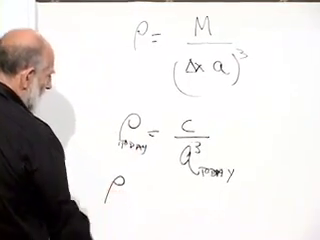
\includegraphics[width=0.72\textwidth]{lecture_09_figure_04.png}
  \caption{Ein Koordinatengitter, das sich mit einem expandierenden räumlichen Tuch mitbewegt.
  Quellbild bei 00:22:20.}
  \label{fig:l09-comoving-grid-board}
\end{figure}

Für zwei Objekte, die entlang der \(x\)-Achse durch ein festes mitbewegtes Intervall \(\Delta x\) getrennt sind, beträgt ihr physikalischer Abstand
\begin{equation}
  D(t)=a(t)\,\Delta x.
  \label{eq:l09-physical-distance}
\end{equation}
Leiten wir ab und halten dabei \(\Delta x\) fest, so erhalten wir
\begin{equation}
  v(t)=\dot a(t)\,\Delta x
      =\frac{\dot a(t)}{a(t)}D(t).
\end{equation}
Definieren wir
\begin{equation}
  H(t)\equiv\frac{\dot a(t)}{a(t)},
  \label{eq:l09-hubble-parameter}
\end{equation}
erhalten wir das Hubble-Gesetz,
\begin{equation}
  v=H(t)D.
  \label{eq:l09-hubble-law}
\end{equation}
Das Wort „konstant“ in „Hubble-Konstante“ bedeutet, dass der Wert zu einem bestimmten kosmischen Zeitpunkt im Raum konstant ist. Es bedeutet nicht, dass er sich im Laufe der kosmischen Geschichte nicht ändert.

\begin{figure}[H]
  \centering
  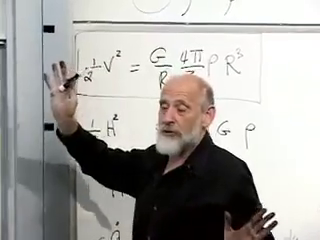
\includegraphics[width=0.72\textwidth]{lecture_09_figure_05.png}
  \caption{Herleitung an der Tafel: \(D=a\Delta x\),
  \(v=(\dot a/a)D=HD\). Quellbild bei 00:26:40.}
  \label{fig:l09-hubble-board}
\end{figure}

\begin{classroomqa}
\audiencequestion{Müsste der aus einer weit entfernten Galaxie ermittelte Hubble-Parameter nicht tatsächlich dem nahebei heute gemessenen Wert entsprechen, wenn wir die Galaxie zu einem früheren Zeitpunkt sehen?}
\lecturerresponse{Nur wenn die Rückblickzeit klein gegenüber dem Alter des Universums ist. Über mäßige Entfernungen ändert sich \(H(t)\) nur wenig, sodass ein einzelner Wert nützlich ist. Bei wirklich kosmologischen Entfernungen sehen wir frühere Epochen; dann müssen die Zeitabhängigkeiten von \(a\) und \(H\) berücksichtigt werden. Das ist ein Grund dafür, dass wir eine dynamische Gleichung für den Skalenfaktor benötigen.}
\end{classroomqa}

\section{Lichtstrahlen in einem expandierenden Koordinatensystem}

\begin{classroomqa}
\audiencequestion{Beeinflusst der Skalenfaktor die Ausbreitung von Licht zwischen weit entfernten Galaxien?}
\lecturerresponse{Ein Lichtstrahl folgt einer lichtartigen Bahn, also gilt \(d\tau=0\). Für einen Strahl, der sich entlang der positiven \(x\)-Achse bewegt, gilt \(dy=dz=0\), und die expandierende Metrik ergibt
\begin{align}
  0&=dt^2-a^2(t)dx^2,
  &dt&=a(t)dx,\notag\\
  &&\frac{dx}{dt}&=\frac{1}{a(t)}.
  \label{eq:l09-null-ray}
\end{align}
Die Koordinatengeschwindigkeit nimmt mit wachsendem \(a(t)\) ab, doch die lokal gemessene Lichtgeschwindigkeit bleibt \(c=1\). Ein festes Koordinatenintervall entspricht einem wachsenden physikalischen Abstand.}
\end{classroomqa}

\begin{figure}[H]
  \centering
  \includegraphics[width=0.72\textwidth]{lecture_09_figure_06.png}
  \caption{Die Nullbedingung und \(dt=a(t)dx\) für die radiale Ausbreitung von Licht.
  Quellbild bei 00:30:54.}
  \label{fig:l09-null-board}
\end{figure}

Man kann Koordinaten wählen, in denen derselbe Sachverhalt wie „Licht wird weiter draußen langsamer“ klingt. Dann werden Längen und Uhren jedoch entsprechend umständlich beschrieben. Die Sprache der expandierenden Räume ist klarer, weil sie die lokale Aussage bewahrt, dass jeder frei fallende Beobachter dieselbe Lichtgeschwindigkeit misst.

\begin{classroomqa}
\audiencequestion{Gibt es Hinweise darauf, dass sich die lokale Lichtausbreitung und die Atomphysik in weit entfernten Galaxien genauso verhalten?}
\lecturerresponse{Operativ sinnvoll sind nur dimensionslose Vergleiche. Man wählt eine atomare Größe als Längeneinheit und eine atomare oder nukleare Periode als Zeiteinheit und fragt dann, wie viele solcher Perioden das Licht benötigt, um die gewählte Länge zu durchqueren. Spektroskopische Beobachtungen stützen die Aussage, dass diese dimensionslosen Verhältnisse in weit entfernten Regionen gleich sind. Die Evidenz ist indirekt, doch genau mit solchen Vergleichen prüft man die Gleichförmigkeit lokaler Naturgesetze.}
\end{classroomqa}

Als das beobachtbare Universum extrem klein war, konnte Licht einen gegebenen physikalischen Bereich, gemessen in der entsprechenden Lichtlaufzeiteinheit, rasch durchqueren. Das bedeutet nicht, dass \(c\) anders war. Es bedeutet, dass der Bereich selbst klein war.

\section{Eine Newtonsche Kugel im Universum}

Nun wenden wir uns von der Kinematik der Dynamik zu. Wir setzen uns in den Ursprung und zeichnen eine Kugel, die groß genug ist, um viele Galaxien und Galaxienhaufen zu umfassen. Auf ihrer Oberfläche wählen wir eine Galaxie aus. In einem homogenen Universum ist die Massenverteilung um uns kugelsymmetrisch, und Newtons Schalentheorem liefert zwei entscheidende Aussagen:
\begin{enumerate}
  \item Die gesamte außerhalb des gewählten Radius kugelsymmetrisch verteilte Materie übt auf die Galaxie an der Kugeloberfläche keine resultierende Newtonsche Kraft aus.
  \item Die gesamte innerhalb der Kugel befindliche Materie wirkt bei dieser radialen Bewegung so, als wäre sie im Mittelpunkt konzentriert.
\end{enumerate}
Wir wählen ein Bezugssystem, in dem wir ruhen; Geschwindigkeiten und Beschleunigungen im folgenden Argument werden also relativ zu uns gemessen.

\begin{figure}[H]
  \centering
  \includegraphics[width=0.72\textwidth]{lecture_09_figure_08.png}
  \caption{Die Konstruktion mit dem Schalentheorem: Wir befinden uns im Mittelpunkt, eine Testgalaxie liegt auf der Oberfläche einer großen homogenen Kugel. Quellbild bei 00:41:10.}
  \label{fig:l09-shell-board}
\end{figure}

\begin{figure}[H]
  \centering
  \begin{tikzpicture}[scale=0.92,>=Latex]
    \draw[thick] (0,0) circle (2.35);
    \fill (0,0) circle (2pt) node[below left] {us};
    \fill (2.35,0) circle (2.2pt) node[right] {test galaxy \(m\)};
    \draw[->,thick,blue!65!black] (0.18,0) -- (2.15,0)
      node[midway,above] {\(R=a(t)x\)};
    \draw[->,thick,red!65!black] (2.35,0.12) -- (3.25,0.12)
      node[midway,above] {\(v=\dot a(t)x\)};
    \node[align=center,text width=7cm] at (0,-2.85)
      {outside shells cancel;\\enclosed mass acts at the center};
  \end{tikzpicture}
  \caption{Saubere Rekonstruktion der Newtonschen Konstruktion.}
  \label{fig:l09-shell-clean}
\end{figure}

Hat die Galaxie die feste mitbewegte Koordinate \(x\), so sind ihr physikalischer Radius und ihre Geschwindigkeit
\begin{equation}
  R(t)=x a(t),
  \qquad
  v(t)=x\dot a(t)=H(t)R(t).
  \label{eq:l09-radius-velocity}
\end{equation}
Sei \(M\) die innerhalb der Kugel eingeschlossene Masse und \(m\) die Masse der Testgalaxie. Die Newtonsche Energie lautet
\begin{equation}
  E=\frac12 m v^2-\frac{GMm}{R}.
  \label{eq:l09-newtonian-energy}
\end{equation}

\begin{figure}[H]
  \centering
  \includegraphics[width=0.72\textwidth]{lecture_09_figure_09.png}
  \caption{Die vollständige Tafelabfolge \(R=xa\), \(v=x\dot a\) und die Newtonsche Energiegleichung für den Spezialfall \(E=0\). Quellbild bei 00:48:40.}
  \label{fig:l09-energy-board}
\end{figure}

Die Energie kann positiv, null oder negativ sein. Wir beginnen mit dem Grenzfall zwischen Entkommen und erneutem Kollaps, \(E=0\), für den gilt
\begin{equation}
  \frac12 v^2=\frac{GM}{R}.
  \label{eq:l09-zero-energy}
\end{equation}

\begin{classroomqa}
\audiencequestion{Was bedeutet eine Gesamtenergie von null für die sich entfernende Galaxie?}
\lecturerresponse{Das ist genau der Fall mit Fluchtgeschwindigkeit. Positive Energie bedeutet eine Bewegung oberhalb der Fluchtgeschwindigkeit; negative Energie bedeutet eine Bewegung unterhalb der Fluchtgeschwindigkeit und führt im Newtonschen Bild mit Materie allein schließlich zur Rückkehr. Wir beginnen an der Grenze zwischen diesen Möglichkeiten und kehren nach der Herleitung der Gleichung für den flachen Fall zu den anderen Vorzeichen zurück.}
\end{classroomqa}

\begin{classroomqa}
\audiencequestion{Ändert sich die eingeschlossene Masse \(M\), wenn sich die Kugel ausdehnt?}
\lecturerresponse{Nein. Die Kugel bewegt sich mit, sodass dieselben Teilchen in ihr bleiben. Ihr physikalisches Volumen wächst und ihre Dichte sinkt, doch ihre gesamte eingeschlossene Masse bleibt konstant. Diese Unterscheidung zwischen \(M\) und \(\rho(t)\) ist wesentlich.}
\end{classroomqa}

Bei einer homogenen Dichte \(\rho(t)\) gilt
\begin{equation}
  M=\frac{4\pi}{3}\rho(t)R^3.
  \label{eq:l09-enclosed-mass}
\end{equation}
Einsetzen in \eqref{eq:l09-zero-energy} ergibt
\begin{equation}
  \frac12 v^2
  =\frac{G}{R}\left(\frac{4\pi}{3}\rho R^3\right).
  \label{eq:l09-enclosed-energy}
\end{equation}

\begin{figure}[H]
  \centering
  \includegraphics[width=0.72\textwidth]{lecture_09_figure_10.png}
  \caption{Einsetzen der eingeschlossenen Masse in die Gleichung für Energie von null.
  Quellbild bei 00:54:16.060.}
  \label{fig:l09-enclosed-mass-board}
\end{figure}

Mit \(v=HR\) erhalten wir
\begin{align}
  \frac12 H^2R^2
    &=\frac{4\pi G}{3}\rho R^2,\\
  H^2
    &=\frac{8\pi G}{3}\rho.
\end{align}
Damit lautet das Expansionsgesetz für den Fall null Energie und räumlicher Flachheit
\begin{equation}
  \boxed{\left(\frac{\dot a}{a}\right)^2
  =\frac{8\pi G}{3}\rho(t)}.
  \label{eq:l09-flat-friedmann}
\end{equation}
Dass sich \(R^2\) herauskürzt, ist kein Zufall. In einem homogenen Universum muss \(H(t)\) denselben Wert haben, unabhängig davon, welche mitbewegte Galaxie als Testobjekt gewählt wurde.

\begin{figure}[H]
  \centering
  \includegraphics[width=0.72\textwidth]{lecture_09_figure_11.png}
  \caption{Die Kürzung des Radius und die daraus folgende Friedmann-Beziehung für den flachen Fall an der Tafel. Quellbild bei 00:57:30.}
  \label{fig:l09-friedmann-board}
\end{figure}

\begin{classroomqa}
\audiencequestion{Gibt es Hinweise auf die Beziehung für den Fall null Energie?}
\lecturerresponse{Beide Seiten lassen sich aus Beobachtungen erschließen: \(H\) aus Daten zur Rezessionsgeschwindigkeit und \(\rho\), indem man Sterne, Gas, Dunkle Materie und Vakuumenergie berücksichtigt. Der Vergleich zur Zeit der Vorlesung ergab, dass beide Seiten auf etwa ein Prozent genau übereinstimmen. Die Einschränkung ist wichtig: Es müssen alle Energieformen berücksichtigt werden, und die spätere Diskussion der Vakuumenergie verändert die naive Deutung anhand der Fluchtgeschwindigkeit.}
\end{classroomqa}

In Einheiten \(c=1\) haben Massendichte und Energiedichte dieselbe Einheit. Das Symbol \(\rho\) bezeichnet daher die gesamte Energiedichte der jeweils betrachteten Komponente.

\section{Gewöhnliche Materie und das Zweidrittelgesetz}

Gleichung \eqref{eq:l09-flat-friedmann} ist erst dann vollständig, wenn wir wissen, wie sich \(\rho(t)\) ändert. Füllen wir zunächst einen mitbewegten Quader mit langsam bewegten, nichtrelativistischen Teilchen. Seine Koordinatenabmessungen bleiben fest, während sein physikalisches Volumen wie folgt wächst:
\begin{equation}
  V(t)=a^3(t)\,\Delta x\,\Delta y\,\Delta z.
\end{equation}
Teilchenzahl und Ruhemasse im Quader bleiben konstant, also gilt
\begin{equation}
  \rho_{\mathrm m}(t)=\frac{C_{\mathrm m}}{a^3(t)}.
  \label{eq:l09-matter-dilution}
\end{equation}
Normiert auf die heutige Epoche \(t_0\) ergibt sich
\begin{equation}
  \frac{\rho_{\mathrm m}(t)}{\rho_{\mathrm m,0}}
  =\left(\frac{a_0}{a(t)}\right)^3.
  \label{eq:l09-matter-normalized}
\end{equation}

\begin{figure}[H]
  \centering
  \includegraphics[width=0.72\textwidth]{lecture_09_figure_12.png}
  \caption{Materiedichte, ihre Abnahme wie \(a^{-3}\) und Normierung auf den heutigen Wert. Quellbild bei 01:04:47.940.}
  \label{fig:l09-density-board}
\end{figure}

\begin{classroomqa}
\audiencequestion{Wie groß ist ungefähr die heutige Energiedichte des Universums, und können gewöhnliche Atome allein sie liefern?}
\lecturerresponse{Eine Zählung der sichtbaren baryonischen Materie liefert nur einen Teil der Antwort. Dunkle Materie und Dunkle Energie müssen ebenfalls als äquivalente Masse-Energie berücksichtigt werden. Die Vorlesung nennt als grobe Größenordnung einen Wert zwischen einem Atom und einigen Dutzend Wasserstoffmassen-Äquivalenten pro Kubikmeter. Dabei geht es um die Größenordnung, nicht um eine präzise Bestandsaufnahme.}
\end{classroomqa}

Setzen wir \eqref{eq:l09-matter-dilution} in \eqref{eq:l09-flat-friedmann} ein und fassen alle zeitunabhängigen Faktoren in einer positiven Konstanten \(C\) zusammen:
\begin{equation}
  \left(\frac{\dot a}{a}\right)^2=\frac{C}{a^3},
  \qquad
  \dot a^2=\frac{C}{a}.
  \label{eq:l09-matter-ode}
\end{equation}
Es gibt zwei anschauliche Lösungswege. Ein Potenzansatz \(a=K t^p\) verlangt
\begin{equation}
  p-1=-\frac{p}{2},
  \qquad p=\frac23.
\end{equation}
Alternativ integrieren wir den expandierenden Ast der Quadratwurzel:
\begin{equation}
  a^{1/2}\frac{da}{dt}=\sqrt C,
  \qquad
  \int a^{1/2}da=\sqrt C\int dt,
\end{equation}
Nach Wahl des Zeitursprungs beim Urknall folgt daher
\begin{equation}
  a^{3/2}\propto t,
  \qquad
  \boxed{a(t)\propto t^{2/3}}.
  \label{eq:l09-matter-solution}
\end{equation}
Bei der Herleitung an der Tafel geht beim Abgleich der Koeffizienten vorübergehend ein Faktor verloren; durch Rückkehr zum Integral wird der Exponent anschließend überprüft. Die Notizen halten diese Kontrolle fest, zeigen aber nur die korrigierte Rechnung.

\begin{figure}[H]
  \centering
  \includegraphics[width=0.72\textwidth]{lecture_09_figure_13.png}
  \caption{Der Potenzansatz und der eingerahmte Exponent \(p=2/3\). Quellbild
  bei 01:13:05.}
  \label{fig:l09-matter-solution-board}
\end{figure}

Durch Ableiten der Lösung erhalten wir
\begin{equation}
  H(t)=\frac{\dot a}{a}=\frac{2}{3t}.
  \label{eq:l09-matter-hubble}
\end{equation}
In der Vergangenheit war der Hubble-Parameter größer. Wenn man also weit genug zurückblickt, um eine beträchtliche Rückblickzeit zu erreichen, sollte man die lokale lineare Beziehung nicht mit dem heutigen Wert von \(H_0\) unverändert fortschreiben.

\begin{figure}[H]
  \centering
  \includegraphics[width=0.72\textwidth]{lecture_09_figure_14.png}
  \caption{Für \(\dot a/a\) und \(a\propto t^{2/3}\) ergibt sich
  \(H=2/(3t)\). Quellbild bei 01:20:42.}
  \label{fig:l09-hubble-time-board}
\end{figure}

\section{Energievorzeichen und räumliche Krümmung}

Mit Newtonscher Argumentation haben wir den flachen Fall mit Gesamtenergie null hergeleitet. Die Allgemeine Relativitätstheorie fügt eine Tatsache hinzu, die sich nicht allein aus dem Schalentheorem gewinnen lässt: Das Vorzeichen der spezifischen Energie im Newtonschen Sinn entspricht dem Vorzeichen der räumlichen Krümmung.
\begin{center}
\begin{tabular}{@{}>{\raggedright\arraybackslash}p{0.20\linewidth}
                    >{\raggedright\arraybackslash}p{0.29\linewidth}
                    >{\raggedright\arraybackslash}p{0.37\linewidth}@{}}
  \toprule
  Gesamt\-energie & Räumliche Krümmung & Entwicklung bei Materie allein \\
  \midrule
  positiv & negativ (offen) & expandiert für immer \\
  null & null (flach) & nähert sich der Fluchtgrenze \\
  negativ & positiv (geschlossen) & expandiert, erreicht einen Umkehrpunkt und kollabiert erneut \\
  \bottomrule
\end{tabular}
\end{center}
Die letzte Spalte setzt Vakuumenergie gleich null voraus. In der Analogie mit einem Geschoss bedeutet positive Energie eine Geschwindigkeit oberhalb der Fluchtgeschwindigkeit, Energie von null genau die Fluchtgeschwindigkeit und negative Energie eine Geschwindigkeit darunter. Einsteins Gleichungen ordnen diesen drei Fällen jeweils eine offene, flache und geschlossene räumliche Geometrie zu.

\section{Photonen und das Halbgesetz}

Das Materiegesetz \(\rho\propto a^{-3}\) setzt voraus, dass die Energie jedes Teilchens näherungsweise konstant bleibt, während die Teilchenzahldichte abnimmt. Für Photonen gilt diese Annahme nicht. Für ein Photon gilt
\begin{equation}
  E=h\nu=\frac{hc}{\lambda}.
\end{equation}
Durch die Expansion wird seine Wellenlänge proportional zum Skalenfaktor gestreckt:
\begin{equation}
  \lambda\propto a,
  \qquad E\propto a^{-1}.
\end{equation}
Die Photonenzahldichte nimmt weiterhin wie \(a^{-3}\) ab, und die Energie jedes Photons bringt einen zusätzlichen Faktor \(a^{-1}\) ein. Daher gilt
\begin{equation}
  \boxed{\rho_{\mathrm r}(t)\propto a^{-4}(t)}.
  \label{eq:l09-radiation-dilution}
\end{equation}

Die Analogie mit einer Gitarrensaite veranschaulicht das physikalische Bild. Zupft man eine Saite an und verlängert dann den schwingenden Abschnitt, wird die Wellenlänge größer und der Ton tiefer. Eine Photonenmode in einem expandierenden mitbewegten Kasten verhält sich ähnlich. Betrachtet man den Vorgang rückwärts, verkürzt die Kompression die Wellenlängen und erhöht die Photonenergien.

\begin{figure}[H]
  \centering
  \includegraphics[width=0.72\textwidth]{lecture_09_figure_15.png}
  \caption{Die Beziehung für die Materiedichte wird an der Tafel auf die Skalierung der Strahlung \(\rho_{\mathrm r}\propto a^{-4}\) erweitert. Quellbild bei 01:29:20.}
  \label{fig:l09-radiation-board}
\end{figure}

Setzen wir \(\rho_{\mathrm r}\propto a^{-4}\) in die Friedmann-Gleichung für den flachen Fall ein, erhalten wir
\begin{equation}
  \left(\frac{\dot a}{a}\right)^2=\frac{C_{\mathrm r}}{a^4},
  \qquad
  \dot a\propto a^{-1},
\end{equation}
und damit
\begin{equation}
  \boxed{a(t)\propto t^{1/2}}.
  \label{eq:l09-radiation-solution}
\end{equation}
Das wächst langsamer als \(t^{2/3}\). Weit genug in der Vergangenheit muss die Strahlung gegenüber gewöhnlicher Materie dominieren, denn \(a^{-4}\) nimmt bei abnehmendem \(a\) schneller zu als \(a^{-3}\). Der Übergang zwischen Materie- und Strahlungsdominanz liegt der Vorlesung zufolge ungefähr in der Epoche, in der der Skalenfaktor etwa tausendmal kleiner war als heute. Davor dominierte die Strahlung, danach über einen langen Zeitraum die Materie.

\section{Vakuumenergie und exponentielle Expansion}

Vakuumenergie skaliert entgegengesetzt. Ihre Dichte ist eine Eigenschaft des leeren Raums und nimmt bei der Expansion des Universums nicht ab:
\begin{equation}
  \rho_\Lambda=\text{constant}.
  \label{eq:l09-vacuum-density}
\end{equation}
Gewöhnliche Materie und Strahlung werden in der Vergangenheit dichter, während dieser Beitrag sich nicht ändert. Deshalb war er im frühen Universum weniger wichtig und gewinnt an Bedeutung, wenn die anderen Komponenten verdünnt werden. Die Vorlesung verwendet die damalige Schätzung, dass Vakuumenergie etwa \(70\%\) der heutigen kosmischen Energiedichte ausmacht.

Bei konstantem \(\rho_\Lambda\) ergibt Gleichung \eqref{eq:l09-flat-friedmann} eine konstante Expansionsrate:
\begin{equation}
  H_\Lambda=\sqrt{\frac{8\pi G}{3}\rho_\Lambda},
  \qquad
  \frac{\dot a}{a}=H_\Lambda.
\end{equation}
Daher gilt
\begin{equation}
  \boxed{a(t)=a(t_i)e^{H_\Lambda(t-t_i)}}.
  \label{eq:l09-vacuum-solution}
\end{equation}

\begin{figure}[H]
  \centering
  \includegraphics[width=0.72\textwidth]{lecture_09_figure_16.png}
  \caption{Die Gleichung mit konstanter Dichte führt zur exponentiellen Expansion.
  Quellbild bei 01:35:48.}
  \label{fig:l09-vacuum-board}
\end{figure}

Bei der in der Vorlesung genannten beobachteten Größenordnung verdoppelt sich die lineare Größe des Universums in etwa zehn bis zwölf Milliarden Jahren. Der Ursprung dieser kleinen, aber von null verschiedenen Vakuumdichte ist weiterhin ungeklärt; ihre Existenz und ihre Wirkung auf die Expansion sind empirische Tatsachen.

\begin{classroomqa}
\audiencequestion{Ist Vakuumenergie in dieser Diskussion dasselbe wie Dunkle Energie?}
\lecturerresponse{Ja. Hier bezeichnet „Dunkle Energie“ eine konstante Vakuumenergiedichte, gleichbedeutend mit einer kosmologischen Konstante. Allgemeinere Modelle mit zeitabhängiger Dunkler Energie sind denkbar, gehören aber nicht zu den Berechnungen dieser Vorlesung.}
\end{classroomqa}

\section{Wie die Expansion des Universums Licht rotverschiebt}

\begin{classroomqa}
\audiencequestion{Wie können Photonen wissen, dass wir expandierende mitbewegte Koordinaten gewählt haben, und deshalb ihre Energie verringern?}
\lecturerresponse{Sie reagieren nicht auf unsere Koordinatenbezeichnungen. Sie breiten sich durch eine Geometrie aus, in der sich die physikalischen Abstände ändern. Ein Wellenzug, der einen Bereich einnimmt, dessen physikalische Größe sich verdoppelt, erhält die doppelte Wellenlänge. Die mitbewegten Koordinaten beschreiben diese Streckung lediglich auf ökonomische Weise; sie verursachen sie nicht.}
\end{classroomqa}

\begin{classroomqa}
\audiencequestion{Woher stammen die Hintergrundphotonen, die uns heute erreichen?}
\lecturerresponse{Je weiter wir in die Ferne blicken, desto weiter blicken wir in die Vergangenheit. Schließlich sehen wir die Epoche, in der das kosmische Material ein ionisiertes Plasma war, undurchsichtig, weil Photonen wiederholt an freien geladenen Teilchen gestreut wurden. Die Grenze, von der aus Photonen zuletzt ungehindert zu uns gelangen konnten, erscheint als eine den Beobachter umgebende Kugel: die Oberfläche der letzten Streuung.}
\end{classroomqa}

\begin{figure}[H]
  \centering
  \includegraphics[width=0.72\textwidth]{lecture_09_figure_17.png}
  \caption{Skizze der beobachterzentrierten Oberfläche der letzten Streuung und immer weiter entfernter Schalen. Quellbild bei 01:42:05.}
  \label{fig:l09-last-scattering-board}
\end{figure}

\begin{figure}[H]
  \centering
  \begin{tikzpicture}[scale=0.9,>=Latex]
    \fill (0,0) circle (2pt) node[below] {observer};
    \draw[thick,orange!70!black] (0,0) circle (2.55);
    \node[orange!70!black,align=center] at (0,3.05)
      {surface of last scattering};
    \foreach \a in {25,75,145,210,285,335}{
      \draw[->,blue!60!black] ({2.55*cos(\a)},{2.55*sin(\a)}) --
        ({1.7*cos(\a)},{1.7*sin(\a)});
    }
    \draw[decorate,decoration={snake,amplitude=1.5pt,segment length=7pt},
      red!65!black,thick,->] (-2.5,0) -- (-0.15,0);
    \node[red!65!black,below] at (-1.35,-0.15)
      {redshifted photon};
  \end{tikzpicture}
  \caption{Saubere Rekonstruktion der Darstellung der letzten Streuung.}
  \label{fig:l09-last-scattering-clean}
\end{figure}

Die Strahlung wurde mit einem für heißes Plasma charakteristischen Spektrum emittiert und erreicht uns mit Wellenlängen, die ungefähr tausendmal länger sind. In der Doppler-Sprache der Vorlesung entfernt sich die weit entfernte emittierende Oberfläche rasch, sodass ihre Strahlung stark rotverschoben ist. In der geometrischen Beschreibung wird die Welle während ihrer Ausbreitung gestreckt. Beide Bilder drücken denselben Zusammenhang aus:
\begin{equation}
  1+z=\frac{\lambda_0}{\lambda_{\mathrm{em}}}
      =\frac{a_0}{a_{\mathrm{em}}}.
  \label{eq:l09-cosmological-redshift}
\end{equation}
\editorialnote{Gleichung \eqref{eq:l09-cosmological-redshift} ist die übliche quantitative Form der Streckungs- und Doppler-Beschreibungen aus der Vorlesung.}

Zu einer früheren Beobachtungsepoche wäre die Oberfläche der letzten Streuung im entsprechenden Bild näher gewesen; die beobachteten Hintergrundphotonen wären weniger rotverschoben und damit energiereicher gewesen. Mit fortschreitender kosmischer Zeit haben die Photonen, die einen mitbewegten Beobachter aus jenem frühen Plasma erreichen, immer längere Wellenlängen.

\section{Wohin geht die Energie eines rotverschobenen Photons?}

\begin{classroomqa}
\audiencequestion{Ein Photon wird mit der Energie \(h\nu_{\mathrm{em}}\) emittiert und kommt rotverschoben mit geringerer Energie an. Was ist mit der Energiedifferenz geschehen?}
\lecturerresponse{Die Newtonsche Herleitung begann mit einer Energiegleichung. Ihre kosmologische Form verknüpft die Expansionsrate mit der Energie­dichte der Materie, sodass Materieenergie und Expansion nicht als unabhängig voneinander erhaltene Größen behandelt werden können. Der Vorlesung zufolge geht die verlorene Photonenenergie in die Energiebilanz der Expansion ein. Ein mit Strahlung gefüllter Kolben veranschaulicht die Analogie: Der Strahlungsdruck schiebt den Kolben nach außen, die Photonenwellenlängen nehmen zu, und ihre verlorene Energie wird zu mechanischer Arbeit und kinetischer Energie des Kolbens.}
\end{classroomqa}

\begin{figure}[H]
  \centering
  \includegraphics[width=0.72\textwidth]{lecture_09_figure_18.png}
  \caption{Die eingerahmte Newtonsche Energiegleichung steht an der Tafel über der entsprechenden Friedmann-Gleichung. Quellbild bei 01:44:42.}
  \label{fig:l09-energy-bookkeeping-board}
\end{figure}

\begin{classroomqa}
\audiencequestion{Was koppelt die Strahlungsenergie an die Expansion?}
\lecturerresponse{Der Druck. In einem Zylinder mit beweglichem Kolben übertragen Photonen Impuls auf die Wand. Bewegt sich der Kolben, verrichtet die Strahlung Arbeit; ihre Wellenlänge wächst und ihre Energie nimmt ab. Das homogene expandierende Universum hat keinen tatsächlichen äußeren Kolben, doch die Analogie mit \(p\,dV\) erklärt, warum die Energiedichte der Strahlung schneller abnimmt, als es allein durch die abnehmende Teilchenzahldichte der Fall wäre.}
\end{classroomqa}

\begin{figure}[H]
  \centering
  \includegraphics[width=0.72\textwidth]{lecture_09_figure_19.png}
  \caption{Der bewegliche, mit Photonen gefüllte Kolben veranschaulicht die Druckarbeit.
  Quellbild bei 01:46:40.}
  \label{fig:l09-piston-board}
\end{figure}

\begin{figure}[H]
  \centering
  \begin{tikzpicture}[scale=0.92,>=Latex]
    \draw[thick] (0,0) rectangle (5.3,2.6);
    \draw[very thick] (4.25,0) -- (4.25,2.6);
    \draw[very thick] (4.25,1.3) -- (5.25,1.3);
    \draw[->,thick,red!65!black] (5.25,1.3) -- (6.2,1.3)
      node[right] {moving piston};
    \foreach \y in {0.55,1.3,2.05}{
      \draw[decorate,decoration={snake,amplitude=1.4pt,segment length=6pt},
        blue!65!black,->] (0.35,\y) -- (3.9,\y);
    }
    \node at (2.15,-0.45) {radiation does \(p\,dV\) work};
  \end{tikzpicture}
  \caption{Saubere Rekonstruktion der Kolbenanalogie für Strahlung.}
  \label{fig:l09-piston-clean}
\end{figure}

Energie erfordert in der allgemeinen Relativitätstheorie besondere Sorgfalt. In einer allgemeinen expandierenden Raumzeit muss es keine eindeutige globale Erhaltungsgröße geben, die der Energie eines isolierten Newtonschen Systems entspricht. Die lokale Erhaltung des Energie-Impuls-Tensors gilt weiterhin; für ein homogenes Fluid führt sie zur Kontinuitätsgleichung
\begin{equation}
  \dot\rho+3H(\rho+p)=0,
  \label{eq:l09-continuity}
\end{equation}
Sie enthält den Druckarbeits-Term, der den Skalierungsgesetzen für Materie und Strahlung zugrunde liegt.\editorialnote{Gleichung \eqref{eq:l09-continuity} ist die präzise lokale Aussage der allgemeinen Relativitätstheorie, auf der die bewusst Newtonsche Analogie der Vorlesung zur Energiebilanz beruht.}

Vakuumenergie macht das Rätsel besonders deutlich. Da ihre Dichte konstant bleibt, während das Volumen wächst, nimmt die gesamte Vakuumenergie in einem mitbewegten Gebiet zu. Ihr negativer Druck ist Teil der Gravitationsquelle und treibt die beschleunigte Expansion an. Man sollte daher nicht die separate Erhaltung der naiven „Materieenergie in einem mitbewegten Kasten“ fordern, ohne Geometrie und Druckarbeit einzubeziehen.

\section{Warum sich der Skalenfaktor aus dem Zeitterm entfernen lässt}

\begin{classroomqa}
\audiencequestion{Warum multipliziert der Skalenfaktor den räumlichen Teil der Metrik, aber nicht den zeitlichen?}
\lecturerresponse{Das ist eine Wahl der Zeitkoordinate. Nehmen wir an, man beginnt mit der konformen Zeitkoordinate \(t\), für die gilt:
\begin{equation}
  d\tau^2=A^2(t)\left(dt^2-dx^2\right).
\end{equation}
Nun definieren wir eine neue kosmische Zeit \(T\) durch
\begin{equation}
  dT=A(t)\,dt.
\end{equation}
Dann gilt:
\begin{equation}
  d\tau^2=dT^2-A^2\bigl(t(T)\bigr)dx^2.
\end{equation}
Der gemeinsame Faktor vor dem Zeitdifferential ist verschwunden, während der physikalische Skalenfaktor im räumlichen Term erhalten bleibt.}
\end{classroomqa}

\begin{figure}[H]
  \centering
  \includegraphics[width=0.72\textwidth]{lecture_09_figure_20.png}
  \caption{Die Zeitumparametrisierung \(dT=A(t)dt\), mit der konforme Zeit in kosmische Zeit umgewandelt wird. Quellbild bei 01:51:05.}
  \label{fig:l09-time-reparam-board}
\end{figure}

\section{Krümmung, Vakuumenergie und das Schicksal des Kosmos}

\begin{classroomqa}
\audiencequestion{Wenn das Universum positiv gekrümmt wäre, müssten wir dann nicht bereits Galaxien auf uns zukommen sehen?}
\lecturerresponse{Nicht unbedingt. Ein Geschoss, das mit einer Geschwindigkeit unterhalb der Fluchtgeschwindigkeit gestartet wird, bewegt sich zunächst nach außen, erreicht einen Umkehrpunkt und fällt erst danach zurück. Wir beobachten das Universum während einer Expansionsphase. Ohne Vakuumenergie würde ein positiv gekrümmtes, von Materie dominiertes Universum schließlich wieder kollabieren. Eine hinreichend große positive Vakuumenergie verhindert diese Umkehr, und ihr beobachteter Wert scheint groß genug zu sein, um die Expansion langfristig unabhängig von einer geringen räumlichen Krümmung exponentiell werden zu lassen.}
\end{classroomqa}

Die exponentielle Zukunft ist kein energetisches Paradies. Sterne erlöschen schließlich, die Dichten von Materie und Strahlung nehmen exponentiell ab, und weit voneinander entfernte Gebiete verlieren den kausalen Kontakt. Die Vakuumenergie bleibt bestehen, während gewöhnliche Strukturen zunehmend kälter und dünner verteilt werden.

\begin{classroomqa}
\audiencequestion{Gibt es in der weiter zurückliegenden Vergangenheit mehr Photonen als gewöhnliche Teilchen?}
\lecturerresponse{Das Verhältnis der Photonenzahl zur Baryonenzahl ist bereits enorm; in der Schätzung der Vorlesung kommen ungefähr \(10^{10}\) Photonen auf ein Baryon. Beide Zahlen bleiben in einem mitbewegten Volumen näherungsweise konstant. In der Vergangenheit ändert sich vor allem die Energie pro Photon. Die Photonenergien steigen wie \(a^{-1}\), die Ruhemasse nichtrelativistischer Teilchen dagegen nicht. Daher dominiert Strahlung zu frühen Zeiten die Energiedichte, auch wenn sich das Zahlenverhältnis selbst nicht ändern muss.}
\end{classroomqa}

Die zentrale Erkenntnis lautet, dass die Geometrie allein die kosmische Entwicklung nicht bestimmt. Die flache Friedmann-Gleichung stellt den Zusammenhang zwischen Expansion und Energiedichte her, doch der Materieinhalt bestimmt deren zeitliche Entwicklung. Nichtrelativistische Materie ergibt \(a\propto t^{2/3}\), Strahlung ergibt \(a\propto t^{1/2}\), und konstante Vakuumenergie führt zu exponentieller Expansion. Diese drei Gesetze ordnen die aufeinanderfolgenden Epochen des Universums und erklären, warum derselbe Skalenfaktor Abstände, Rotverschiebungen und den sich ändernden Hubble-Parameter bestimmt.
